\documentclass[notitlepage, hidelinks]{article}
\usepackage{natbib}
\usepackage{graphicx}
\usepackage{enumerate}
\usepackage{geometry}
\usepackage{titlesec}
\usepackage{float}
\usepackage{tabularx}
\usepackage[font=footnotesize,labelfont=bf]{caption}
\usepackage{fancyvrb}
\usepackage[ngerman]{babel}
\usepackage{ifxetex,ifluatex}
\usepackage{etoolbox}
\usepackage[svgnames]{xcolor}
\usepackage{tikz}
\usepackage{xcolor}
\usepackage{multirow}
\usepackage{color, colortbl}
\usepackage{wrapfig}
\usepackage{changepage}
\usepackage{listings}
\usepackage[hyphens]{url}
\usepackage{hyperref}
\usepackage{tikz}
\usepackage{caption}
\newcommand\ytl[2]{
\parbox[b]{16em}{\hfill{\color{black}\bfseries #1}~$\cdots\cdots$~}\makebox[0pt][c]{$\bullet$}\vrule\quad \parbox[c]{14.5cm}{\vspace{10pt}\color{black}\raggedright #2.\\[10pt]}\\[-3pt]
}

\definecolor{Gray}{gray}{0.75}
\definecolor{LightGray}{gray}{0.9}

\definecolor{red}{rgb}{0,0.2,0.701} 
\definecolor{blue}{rgb}{0.023,0.49,0.0117}
\definecolor{green}{rgb}{0,0.8,0}
\definecolor{cyan}{rgb}{0.0,0.38,0.51}
\definecolor{cloudwhite}{rgb}{1, 1, 1}
\definecolor{black}{rgb}{0,0,0}
\definecolor{bluebg}{rgb}{0.05,0.278,0.63}

\lstset{
language=csh,
basicstyle=\footnotesize\ttfamily,
numbers=left,
numberstyle=\tiny,
numbersep=5pt,
tabsize=1,
extendedchars=true,
breaklines=true,
frame=b,
stringstyle=\color{blue}\ttfamily,
showspaces=false,
showtabs=false,
xleftmargin=20pt,
xrightmargin=3pt,
framexleftmargin=17pt,
framexrightmargin=5pt,
framexbottommargin=4pt,
commentstyle=\color{green},
morecomment=[l]{//}, %use comment-line-style!
morecomment=[s]{/*}{*/}, %for multiline comments
showstringspaces=false,
morekeywords={ abstract, event, new, struct,
as, explicit, null, switch,
base, extern, object, this,
bool, false, operator, throw,
break, finally, out, true,
byte, fixed, override, try,
case, float, params, typeof,
catch, for, private, uint,
char, foreach, protected, ulong,
checked, goto, public, unchecked,
class, if, readonly, unsafe,
const, implicit, ref, ushort,
continue, in, return, using,
decimal, int, sbyte, virtual,
default, interface, sealed, volatile,
delegate, internal, short, void,
do, is, sizeof, while,
double, lock, stackalloc,
else, long, static,
enum, namespace, string},
keywordstyle=\color{cyan},
identifierstyle=\color{black},
backgroundcolor=\color{cloudwhite},
}



\DeclareCaptionFont{white}{\color{white}}
\DeclareCaptionFormat{listing}{\colorbox{bluebg}{\parbox{\textwidth}{\hspace{15pt}#1#2#3}}}
\captionsetup[lstlisting]{format=listing,labelfont=white,textfont=white, singlelinecheck=false, margin=0pt, font={bf,footnotesize}}
\lstset{defaultdialect=[Sharp]C}


\setcounter{tocdepth}{5}
\setcounter{secnumdepth}{5}


\usetikzlibrary{backgrounds}
\makeatletter

\tikzset{%
  fancy quotes/.style={
    text width=\fq@width pt,
    align=justify,
    inner sep=1em,
    anchor=north west,
    minimum width=\linewidth,
  },
  fancy quotes width/.initial={.8\linewidth},
  fancy quotes marks/.style={
    scale=8,
    text=gray,
    inner sep=0pt,
  },
  fancy quotes opening/.style={
    fancy quotes marks,
  },
  fancy quotes closing/.style={
    fancy quotes marks,
  },
  fancy quotes background/.style={
    show background rectangle,
    inner frame xsep=0pt,
    background rectangle/.style={
      fill=white!25,
      rounded corners,
    },
  }
}

\newenvironment{fancyquotes}[1][]{%
\noindent
\tikzpicture[fancy quotes background]
\node[fancy quotes opening,anchor=north west] (fq@ul) at (0,0) {``};
\tikz@scan@one@point\pgfutil@firstofone(fq@ul.east)
\pgfmathsetmacro{\fq@width}{\linewidth - 2*\pgf@x}
\node[fancy quotes,#1] (fq@txt) at (fq@ul.north west) \bgroup}
{\egroup;
\node[overlay,fancy quotes closing,anchor=east] at (fq@txt.south east) {''};
\endtikzpicture}


\pgfmathsetmacro{\fq@width}{\linewidth - 2*\pgf@x}


\renewcommand{\figurename}{Abb.}
\geometry{left=3cm, right=3cm, bottom=2cm, top=2.5cm}
\titlespacing*{\section}{0pt}{7ex plus 1ex minus .2ex}{4.3ex plus .2ex}
\titlespacing*{\subsection}{0pt}{7ex plus 1ex minus .2ex}{4.3ex plus .2ex}
\setlength\parindent{0pt}
\newcolumntype{L}[1]{>{\raggedright\let\newline\\\arraybackslash\hspace{0pt}}m{#1}}
\def\changemargin#1#2{\list{}{\rightmargin#2\leftmargin#1}\item[]}
\let\endchangemargin=\endlist 


\begin{document}

\mbox{}\\ \mbox{}\\\mbox{}\\ \mbox{}\\\mbox{}\\ \mbox{}\\\mbox{}\\\mbox{}\\
\mbox{}\\\mbox{}\\\mbox{}\\\mbox{}\\\mbox{}\\\mbox{}\\\mbox{}\\\mbox{}\\
\begin{center}
\huge
\textbf{E-Business Architekturen} \\ 
\LARGE
Prüfungsleistung (Gruppenaufgabe) \\
\mbox{}\\
\large
Ergebnisprotokolle der Komplexübungen 1, 2, 3b und 4d im Rahmen der Veranstaltung E-Business Architekturen  \\

\mbox{}\\ \mbox{}\\
\large
vorgelegt am \\
07.05.2023 \\
\mbox{}\\
an der \\
Hochschule für Wirtschaft und Recht Berlin \\
Fachbereich Duales Studium \\
\end{center}

\mbox{}\\ \mbox{}\\\mbox{}\\ \mbox{}\\\mbox{}\\ \mbox{}\\\mbox{}\\ \mbox{}\\\mbox{}\\ \mbox{}\\
\begin{table}[H]
\begin{tabular}{ l l }
von: 
& Robert Neubert \\
& Danny Neupauer \\
& Hannes Roever \\
Fachrichtung: & Wirtschaftsinformatik \\
Studienjahrgang: & WI20C \\
Studienhalbjahr:& Wintersemester 2022/23 \\
Dozent: & Prof. Dr. Andreas Schmietendorf \\
\end{tabular}
\end{table}

\thispagestyle{empty}
\clearpage
\newpage
\tableofcontents
\thispagestyle{empty}
\clearpage

\normalsize
\pagenumbering{arabic}


\section{Einleitung}
lalala\footnote{Vgl. \cite{athey2018impact}, S.5} und sind insofern für komplexe sozialwissenschaftliche Fragestellungen aufgrund des vorhandenen Bias\footnote{Vgl. \cite{miceli2022studying}, S.3ff} \\
lalalala\footnote{Vgl. \cite{blogKorab}, online}

\section{Aufgabe 1: E-Business Grundlagen}

\subsection{Anwendung des Begriffs E-Business}
Was verbinden Sie mit dem Begriff des E-Business? Versuchen Sie die folgenden Aspekte zu berücksichtigen, nennen Sie ggf. weitere.
\begin{itemize}
\item Organisatorische Aspekte
\item Prozessbezogene Aspekte (z.B. Geschäftsprozess)
\item Technologische Aspekte (z.B. Entwicklung \& Betrieb)
\item Gesellschaftliche Implikationen (z.B. Soziologische Aspekte)
\end{itemize}

\subsection{Beziehung zu domänenspezifischen Lösungen}
Welche Beziehungen sehen Sie zu den folgenden Lösungen?
\begin{itemize}
\item Systeme für das e-Learning (z.B. Moodle oder Open HPI)
\item Systeme für das e-Government (z.B. ELSTER oder Fahrzeugzulassung)
\item Systeme für das e–Banking (z.B. Instant Payment)
\item Systeme für das e-Commerce (z.B. Web Shops)
\end{itemize}

\subsection{Ziele und Erwartungen an E-Business Lösungen}
Welche Ziele und Erwartungen verknüpfen Unternehmen und ihre Kunden mit e-Business-Lösungen?
\begin{itemize}
\item Berücksichtigen sie ggf. unterschiedliche Sichten
\item Nennen Sie ihnen bekannte Lösungen (z.B. aus den Praktika)
\item Identifizieren Sie mögliche Vor- und Nachteile
\end{itemize}

\subsection{Eigenschaften von E-Business Softwarearchitekturen}
Über welche Eigenschaften sollten Softwarearchitekturen für e-Business-Lösungen verfügen?
\begin{itemize}
\item Fragen des Kommunikationssystems
\item Verwendete Rechnerinfrastruktur
\item Eigenschaften entwickelter Softwaresysteme
\end{itemize}

\subsection{E-Business im konkreten Unternehmenskontext}
Wie könnte eine Strategie zur Einführung einer e-Business-Architektur in einem Unternehmen ihrer Wahl aussehen?
\begin{itemize}
\item Notwendige Voraussetzungen \& Rahmenbedingungen
\item Auswirkungen auf das Informationsmanagement (CIO)
\item Auswirkungen auf die Entwicklung von Software (Lösungsanbieter)
\item Auswirkungen auf den Betrieb von Software (Rechenzentren)
\item Mehrwertpotentiale für die Kunden und Lieferanten
\end{itemize}

Worin sehen Sie weitere Aspekte eines digitalen Unternehmens, die mit dem Begriff des e-Business nicht erfasst werden?

\section{Aufgabe 2: Serviceverzeichnisse}
\subsection{Analyse eines Verzeichnisdienstes}
Analysieren Sie die Möglichkeiten eines in Abstimmung mit dem Dozenten zu wählenden Verzeichnisdienstes für Web-APIs.
\begin{itemize}
\item Recherche und Auswahl eines Verzeichnisdienstes:
\begin{itemize}
\item Anzahl und Art der registrierten Web-APIs (ggf. auch Open Data)
\item Allgemeiner Funktionsumfang des Verzeichnisdienstes
\item Hinterlegte Klassifikationen – d.h. Organisation der Serviceablage
\item Vorgehensweise zum ggf. Suchen von Serviceangeboten
\item Vorgehensweise zum ggf. Registrieren eigener Serviceangebote
\item Bereitgestellte Entwicklerunterstützung, wie z.B. Beispielcode
\end{itemize}
\item Voraussetzungen zur Nutzung (Registrierung, Kosten, …)?
\item Vergleich von API- und datenorient. Schnittstellen (z.B. Open Data)?
\end{itemize}

In dieser Unteraufgabe wird sich mit der Nutzung und Analyse von Service-Verzeichnissen beschäftigt. Dazu wird sich zunächst für einen zu betrachtenden Verzeichnisdienst entschieden, welcher im weiteren Verlauf der Aufgabe auf seine Eigenschaften überprüft wird.

\subsubsection{Vorgehensweise bei der Auswahl eines Verzeichnisdienstes}
Um einen vollumfänglichen Überblick über den Verzeichnisdienst bieten zu können, wurde bei der Auswahl des Verzeichnisdienstes darauf geachtet, einen Verzeichnisdienst ohne Zugangsbeschränkungen mit öffentlich zugänglichen APIs zu wählen. Aufgrund dieser Vorgaben wir uns für das API-Verzeichnis des Bundes entschieden. \\
Die APIs, die unter der Webadresse https://bund.dev/apis zusammengefasst sind, dienen dem Zweck, den Zugang zu verschiedenen Datensätzen und Verwaltungsverfahren der Bundesverwaltung zu erleichtern. Sie ermöglichen es Entwicklern und anderen interessierten Nutzern, auf eine standardisierte und dokumentierte Art und Weise auf diese Informationen zuzugreifen und sie in eigenen Anwendungen zu nutzen. Dabei können die APIs verschiedene Funktionalitäten bereitstellen, wie beispielsweise die Abfrage von Daten, die Bearbeitung von Anträgen oder die Einreichung von Dokumenten. Durch die Bereitstellung dieser APIs im Rahmen der Open Government Umsetzungsstrategie des Bundes wird eine transparentere und effizientere Zusammenarbeit zwischen Verwaltung und Bürgern angestrebt.

\subsubsection{Allgemeines über den Verzeichnisdienst}
In ihrer Gesamtheit sind auf der Website insgesamt 47 diverse Web-APIs identifizierbar. Diese APIs können hauptsächlich verschiedenen Bundesbehörden zugeordnet werden. Jedoch lassen sich vereinzelt auch APIs von Landesbehörden sowie von Anstalten des öffentlichen Rechts ausmachen. Für jede der identifizierten APIs existiert eine eigene Dokumentation, welche gegebenenfalls auf GIT Hub oder eine andere Webpräsenz verweist. Innerhalb der Dokumentationen finden sich prägnante Beschreibungen und teilweise auch Verwendungsbeispiele für die jeweilige API.


\begin{figure}[H]
\centering
  
\includegraphics[width=\textwidth]{images/bundwebsite.png}
  \caption{Ansicht der Startseite des Verzeichnisdienstes}
  \label{fig:}
\end{figure}

In diesem Kontext ist die Integration individueller Application Programming Interfaces (APIs) nicht vorgesehen. Ebenso besteht keine Möglichkeit zur Erstellung eigener Code-Zweige sowie der Integration von Eigenprogrammierung. Lediglich die Meldung von Code-Problemen mittels GIT Hub-Funktionalität sowie das durchführen eines Pull Requestes ist gestattet. Bei einigen APIs ist es außerdem möglich, Probleme über alternative Kommunikationskanäle zu melden. Eine standardisierte Vorlage für das Reporting von Schwierigkeiten besteht nicht

\begin{figure}[H]
\centering
  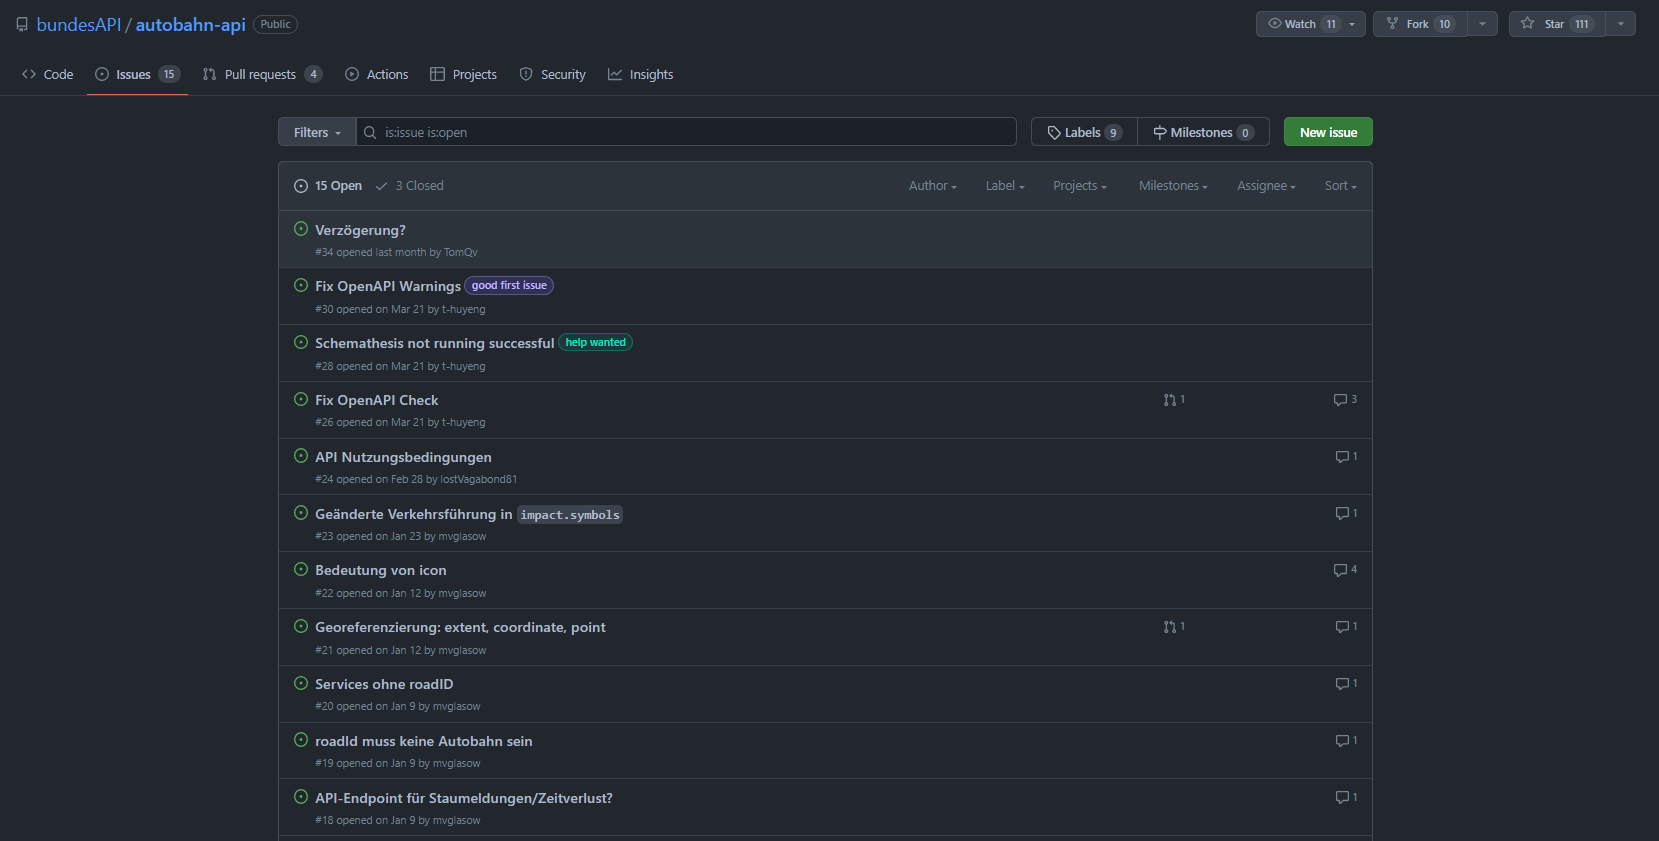
\includegraphics[width=\textwidth]{images/gitissues.png}
  \caption{Gemeldete Probleme}
  \label{fig:gitissues}
\end{figure}

Wie in Abb.\ref{fig:gitissues} ersichtlich ist, können bei der Erstellung von Problemen verschiedene Tags zugeordnet werden, um eine Klassifizierung für den Entwickler zu erleichtern. \\
Der Verzeichnisdienst ist ohne vorherige Anmeldung oder Registrierung zugänglich. Ebenso kann der API-Code ohne GIT-Registrierung oder Anmeldung heruntergeladen werden. Das Melden von Problemen über die GIT-Funktion erfordert jedoch eine vorherige Anmeldung und Registrierung. Analog dazu verhält es sich bei verfügbaren Pull Requests und ähnlichen Funktionalitäten.

\subsubsection{Vergleich von API- und datenorientierten Schnittstellen}
Beide Schnittstellen sind Softwareschnittstellen, die sich in einzelnen Punkten und Funktionalitäten unterscheiden: \\
Eine API (Application Programming Interface) ist eine Art von Schnittstelle, die es Anwendungen ermöglicht, mit anderen Anwendungen, Systemen oder Diensten zu interagieren. Es stellt eine Sammlung von Methoden, Funktionen und Protokollen bereit, die von einer Anwendung aufgerufen werden können, um bestimmte Aktionen auszuführen oder Daten abzurufen. Eine API dient als Abstraktionsschicht, die es einer Anwendung ermöglicht, auf die Funktionalität eines anderen Systems zuzugreifen, ohne dass sie das interne Datenmodell oder die Implementierungsdetails kennen muss. APIs sind in der Regel gut dokumentiert und stellen eine klare Schnittstelle bereit, über die Anwendungen miteinander kommunizieren können. \\
Eine datenorientierte Schnittstelle ist eine Art von Schnittstelle, die es Anwendungen ermöglicht, auf strukturierte oder unstrukturierte Daten zuzugreifen, sie zu manipulieren und zu speichern. Im Gegensatz zu einer API, die eine Sammlung von Methoden und Funktionen bereitstellt, um bestimmte Aktionen auszuführen oder Daten abzurufen, liegt der Schwerpunkt bei einer datenorientierten Schnittstelle auf dem direkten Zugriff auf die Daten selbst. Datenorientierte Schnittstellen können beispielsweise in Form von Datenbankzugriffen oder Dateisystemzugriffen bereitgestellt werden. Im Allgemeinen erfordern sie spezielle Kenntnisse und Fähigkeiten, um sie zu nutzen, und sind oft weniger benutzerfreundlich als APIs.

\begin{table}[h]
\begin{center}
\begin{tabular}{| L{3.1cm} | L{5.6cm} | L{5.6cm} |}
\hline
Kriterium & API-Schnittstelle & Datenschnittstelle \\ \hline
Flexibilität & Hoch & Niedrig \\ 
& APIs bieten in der Regel mehr Flexibilität, da sie in der Lage sind, unterschiedliche Arten von Anwendungen und Plattformen zu bedienen. & Datenorientierte Schnittstellen sind in der Regel weniger flexibel, da sie sich auf spezifische Datenmodelle und -typen konzentrieren. \\ \hline
Sicherheit & Höher & Niedriger \\ 
& APIs bieten in der Regel mehr Sicherheitsfunktionen wie Autorisierung, Authentifizierung und Verschlüsselung. & Datenorientierte Schnittstellen bieten in der Regel weniger Sicherheitsfunktionen, da sie sich auf den Zugriff auf Daten konzentrieren. \\ \hline
Kompatibilität & Hoch & Niedriger \\ 
& APIs sind in der Regel kompatibel mit einer Vielzahl von Plattformen, Sprachen und Systemen. & Datenorientierte Schnittstellen sind in der Regel auf bestimmte Datenquellen oder Datenbanken beschränkt. \\ \hline
Geschwindigkeit & In der Regel Höher & In der Regel niedriger \\ 
& APIs bieten in der Regel schnellere Verarbeitungsgeschwindigkeiten, da sie oft auf leichte und effiziente Übertragung von Daten ausgelegt sind. & Datenorientierte Schnittstellen sind in der Regel langsamer, da sie oft auf komplexe Datenstrukturen und Datenbankabfragen zugreifen müssen. \\ \hline
Verwendung & Für Entwickler und Programmierer & Für Endbenutzer \\ 
Granularität & Höhere Granularität & Geringere Granularität \\ 
& APIs bieten in der Regel eine höhere Granularität, da sie in der Lage sind, einzelne Funktionen und Dienste aufzurufen. & Datenorientierte Schnittstellen bieten in der Regel eine geringere Granularität, da sie sich auf den Zugriff auf bestimmte Datensätze oder Datenquellen konzentrieren. \\ \hline
\end{tabular}
\caption{Vergleich von API-Schnittstellen und Datenschnittstellen}
\label{tab:apis-vs-data-interfaces}
\end{center}
\end{table}

Es ist zu beachten, dass die Unterschiede zwischen den beiden Typen von Schnittstellen nicht immer so klar abgegrenzt sind und dass einige APIs datenorientiert sein können und einige Datenorientierte Schnittstellen APIs-ähnliche Funktionen bieten können.


\subsection{Analyse von Web-APIs}

\subsubsection{Erstellung des Bewertungsmodells}
Erstellen Sie ein Bewertungsmodell für angebotene Web APIs
\begin{itemize}
\item Welche Informationen halten Sie für einen Einsatz notwendig?
\begin{itemize}
\item Spezifikation/Technologie (SOAP, REST, JSON, MIME, …)
\item Servicebeschreibung (technisch \& fachlich)
\item Funktionstüchtigkeit (Qualitätsvereinbarungen)
\item Kontaktinformationen
\item Beispiele zur programmiertechnischen Einbindung
\end{itemize}
\item Informationen zu einem Ansatz für ein Bewertungsmodell – siehe Anlage
\end{itemize}

Wir haben uns dazu entschieden alle API´s aus dem BundDev Verzeichnis zu bewerten. So ist es möglich eine Übersicht der vom Bund bereitgestellten Schnittstellen zu gewinnen. \\
Zu Beginn wurde das Bewertungsmodell in fünf Kategorien aufgeteilt. Diese lauten: Übersicht, Offenheit, Qualität, Dokumentation und Verfügbarkeit.
\begin{enumerate}
\item Übersicht: In diesem Teil wird nur eine Übersicht über die einzelnen API´s dargestellt. Unter welchen URL lässt sich die Dokumentation finden? Wie viele get, post, put, delete und andere werden werden in der API verwendet? Hierbei wird keine Bewertung vorgenommen, sondern es wird nur aufgezählt.
\item Offenheit: 
\begin{itemize}
\item Quellcode: Die Offenlegung des Quellcodes einer API ist ein wichtiger Faktor für die Offenheit einer API, da es Entwicklern ermöglicht, die API zu verstehen, anzupassen und zu erweitern. Wenn der Quellcode einer API offen zugänglich ist, können Entwickler die Funktionalität der API an ihre spezifischen Anforderungen anpassen und Fehler beheben, die in der API auftreten können. Offener Quellcode fördert auch die Zusammenarbeit und Innovation, indem er es anderen Entwicklern ermöglicht, den Code zu überprüfen und Verbesserungen und Erweiterungen vorzuschlagen. Dies kann dazu beitragen, die Qualität und Sicherheit der API zu verbessern.
\item Token/ Registrierung: Eine einfache Registrierung oder Token-Nutzung kann dazu beitragen, die API-Nutzung für die Benutzer zu vereinfachen. Anstatt komplizierte Authentifizierungsmethoden zu verwenden, können Benutzer einfach einen Token generieren oder sich registrieren, um Zugriff auf die API zu erhalten.
\item Zugänglichkeit: Eine offene API sollte für Entwickler leicht zugänglich sein. Die API sollte einfach zu finden und zu registrieren sein, und es sollte keine unnötigen Hürden geben, die die Nutzung der API einschränken.
\item Request Limit: Ein Request-Limit ist eine Einschränkung für die Anzahl der API-Anfragen, die ein Benutzer innerhalb eines bestimmten Zeitraums an den API-Server senden darf. Ein Request-Limit ist wichtig, um die API-Performance, Zuverlässigkeit und Sicherheit zu gewährleisten.
Eine API kann nur eine begrenzte Anzahl von Anfragen gleichzeitig bearbeiten. Wenn zu viele Anfragen gleichzeitig eingehen, kann die API-Performance beeinträchtigt werden. Wenn zu viele Anfragen gleichzeitig eingehen und die API überlasten, kann dies zu Systemausfällen oder Verzögerungen bei der Verarbeitung von Anfragen führen. Einige Benutzer können versuchen, die API durch eine hohe Anzahl von Anfragen zu überlasten, um Schwachstellen auszunutzen oder unerwünschte Aktivitäten durchzuführen. Ein Request-Limit stellt sicher, dass alle Benutzer die gleiche Chance haben, die API zu nutzen.
\item Kontakt: Es ist wichtig, dass zu einer API ein Kontakt hinterlegt ist, damit Benutzer der API einen Ansprechpartner haben, falls sie Fragen oder Probleme haben. Wenn Benutzer auf Probleme bei der Nutzung der API stoßen, können sie sich an den hinterlegten Kontakt wenden, um Hilfe und Unterstützung zu erhalten. Ein Kontakt kann Feedback von den Benutzern der API sammeln und an den API-Anbieter weiterleiten. Dies kann dazu beitragen, die API zu verbessern, indem die Benutzeranforderungen und -bedürfnisse berücksichtigt werden. Ein Kontakt kann dazu beitragen, die Sicherheit der API zu erhöhen, indem er Benutzer über Sicherheitsbedrohungen informiert und sicherstellt, dass diese angemessen behandelt werden.
\end{itemize}
\item Qualität: 
\begin{itemize}
\item Granularität: Die Granularität einer API bezieht sich auf die Anzahl und Komplexität der verfügbaren API-Endpunkte und der darin enthaltenen Funktionalität. Eine API mit zu hoher Granularität enthält möglicherweise zu viele spezialisierte Endpunkte, die für bestimmte Anwendungsfälle entwickelt wurden, während eine API mit zu niedriger Granularität möglicherweise nicht genügend Endpunkte enthält, um die erforderliche Funktionalität bereitzustellen. Es ist daher wichtig, dass die Granularität der API weder zu hoch noch zu niedrig ist.
\item TLS: HTTPS bei einer API eingesetzt wird, um die Sicherheit und Integrität der übertragenen Daten zu gewährleisten. HTTPS ist eine Verschlüsselungsprotokoll, das auf dem HTTP-Protokoll basiert und eine sichere Verbindung zwischen einem Client und einem Server herstellt. TLS ist ein Protokoll, das die Datenverschlüsselung, Authentifizierung und Integritätssicherung während der Übertragung von Daten über ein Netzwerk ermöglicht.
\item Statuscode: Es ist wichtig, dass alle Statuscodes für eine API angegeben sind, da sie den Client über den Zustand der Anfrage informieren und ihm ermöglichen, geeignete Maßnahmen zu ergreifen. Statuscodes sind dreistellige Zahlen, die von einem Server zurückgegeben werden, um den Erfolg oder Misserfolg einer Anfrage anzuzeigen. 
\end{itemize}
\item Dokumentation:
\begin{itemize}
\item Routen: Es ist wichtig, dass alle Routen einer API in der Dokumentation erwähnt sind, um den Entwicklern zu helfen, die API vollständig zu verstehen und korrekt zu nutzen. 
\item Ressourcen: Wenn alle Ressourcen in der Dokumentation erwähnt werden, können Entwickler sicherstellen, dass sie alle verfügbaren Entitäten und Objekte der API verstehen und nutzen. Wenn eine Ressource in der Dokumentation fehlt, kann dies dazu führen, dass Entwickler fehlerhafte Anfragen senden oder unerwartete Ergebnisse erhalten.
\item Parameter: 
\end{itemize}
\item Verfügbarkeit
\end{enumerate}


\subsubsection{Einsatz des Bewertungsmodells}
Analysieren Sie stichpunktartig 20 registrierte Web APIs
\begin{itemize}
\item Verwenden Sie ihr entwickeltes Bewertungsmodell
\item Ausführung der Services mittels Musterlösung (keine Programmierung)
\end{itemize}
Die zu analysierenden Service-APIs sollten möglichst aus unterschiedlichen Serviceverzeichnissen stammen.

\subsection{API - Spezifikationen}
\subsubsection{Spezifikationsanalyse}
Analysieren Sie Struktur und Elemente einer WSDL, OpenAPI-(Swagger) oder auch GraphQL(Schema)-Spezifikation.
\begin{itemize}
\item Verwenden Sie zur Analyse 5 ausgewählte Services
\item Stichpunktartige Beschreibung der Struktur/Unterelemente
\item Metrische Erfassung der Struktur bzw. eingesetzten Elemente
\item Statistische Auswertung Informationen (z.B. Tabellen, Diagramme)
\end{itemize}

\subsubsection{Analysetools}
Nutzen Sie ggf. verfügbare Hilfsmittel und gehen Sie auf die entsprechende Funktionsweise der Tools ein
\begin{itemize}
\item Beispiele: soapUI, SOAPSonar, Postman https://www.postman.com
\item Grafische WSDL-Editoren (z.B. XMLSpy ab Version 8)
\end{itemize}

\subsubsection{Einschränkungen und Alternativen}
\begin{itemize}
\item Welche Informationen fehlen bei der gewählten Spezifikationen?
\item Recherchieren Sie nach alternativen Beschreibungsformen?
\end{itemize}

\section{Übung 3b: Entwicklung eigener Service-Angebote}
\subsection{Möglichkeiten für Implementierung und Deployment}
\subsubsection{Analyse der Möglichkeiten}
Analysieren Sie mit Hilfe des Internets mögliche Alternativen zur Implementierung und Deployment von Web APIs (speziell WSDL/XML, REST/OpenAPI und GraphQL), wie z.B.:
\begin{itemize}
\item IDE NetBeans und GlassFish Server
\item IDE Eclipse und Tomcat \& Axis-Erweiterung
\item Postman API Builder
\item Cloud-basierte Entwicklung/Deployment
\end{itemize}

\subsubsection{Analytischer Vergleich der Möglichkeiten}
Vergleichen Sie die gefunden Alternativen anhand eines eigenen Bewertungsmodells, mit Hilfe von Kriterien wie z.B.:
\begin{itemize}
\item Voraussetzungen zur Verwendung (HW- und SW-Ressourcen)
\item Integration von Entwicklung- und Ausführungsplattform
\item DevOps orientierte Vorgehensweise (Automationsaspekte)
\item Verbreitung, Entwicklersupport, Kosten, Lizenzen
\end{itemize}

\subsection{Entwicklung}
\subsubsection{Rahmenbedingungen}
Wählen Sie für die weiteren Aufgaben dieser Übung eine konkrete Entwicklungsumgebung aus, begründen Sie Ihre Entscheidung
\begin{itemize}
\item Benötigte Softwareversionen und Werkzeuge
\item Installation und Konfiguration der Entwicklungsumgebung
\item Cloud-basierte Implementierung und Betrieb
\end{itemize}
 
 Für eine nachvollziehbare Argumentation, warum der eingesetzte Toolstack verwendet wurde und welche Laufzeitumgebung und Art des Deployments als angebracht eingeschätzt wurde, sollen zunächst kurz die Anforderungen an die Anwendung dargestellt werden. Diese sind zwar ``simuliert'', jedoch (in sehr oberflächlicher Form) an möglichen realen Anforderungen angelehnt. Da die nicht-funktionalen Anforderungen hier eher die Argumentationsgrundlage bilden, stehen diese im Fokus - funktionale Anforderungen sollten nur in Ausnahmefällen eine Determinante für Techstack und Deployment sein.  \\
Überlegungen, welche eine prototypische Umsetzung im gegebenen Rahmen sprengen würden, werden bewusst außer acht gelassen. Dazu gehören: ggfs. initial höhere Entwicklungskosten, verfügbare (Entwicklungs)ressourcen und Skillset der Beteiligten, architektonische Überlegungen und der Einsatz bestimmter Design Patterns, sowie das Thema Tests. \\
Desweiteren halten wir eine Begründung, warum nun welche Entwicklungsumgebung eingesetzt wurde, nicht für sinnvoll. Welche IDE ein Entwickler verwendet, ob als Git nun Github, Gitlab oder Bitbucket verwendet wird und mit welchem Tool REST Endpunkte getestet werden ist entweder von den Vorlieben und Gewohnheiten des Einzelnen abhängig, oder durch Vorgaben des Arbeitgebers bestimmt (oder beides). Insofern beschränken wir uns bei diesen Punkten auf die Benennung der ``Werkzeuge'', ohne das Warum weiter zu vertiefen. Stattdessen wollen wir die aus unserer Sicht viel wichtigere Frage beantworten, warum für den genannten Usecase eine bestimmte Sprache, Bibliotheken und Deploymentszenarien gewählt wurden.
 
\paragraph{Anforderungen} \mbox{} \\

Funktionale Anforderungen:
\begin{itemize}
\item Anzeige von Basisinformationen zu Coderepositories (Autor, Sprache, Forks, Commits), welche über eine REST API abgerufen werden
\item Löschen vorhandener, Hinzufügen neuer und Ändern vorhandener Repositories (Client)
\item Persistierung der Änderungen in einer Datenbank
\item Bereitstellung als Webapp
\end{itemize}

Nicht-funktionale Anforderungen: 
\begin{itemize}
\item unterdurchschnittlich geringe TCO durch:
\begin{itemize}
\item hohe Performanz und geringen Footprint bei der Hardwarenutzung
\item geringe Wartungskosten
\item einfache Verwaltung der Abhängigkeiten
\item einfaches Deployment
\end{itemize}
\item gute Skalierbarkeit
\item hohes Level an Sicherheit
\item volle Flexibilität hinsichtlich der Laufzeitumgebung
\item DB Typ möglichst offen
\end{itemize}



\paragraph{Verwendete Sprache(n)} \mbox{} \\

Client und REST API sollen in Rust geschrieben werden, auch die verwendete Datenbank (Surreal DB) ist in Rust geschrieben. Rust ist eine multi-paradigmatische, noch recht junge (2015) Programmiersprache, die auf konzeptioneller Ebene einige Besonderheiten aufweist. Im Folgenden werden einige dieser Besonderheiten erläutert:
\begin{itemize}
\item Memory-Safety und Thread-Safety: Rust erreicht dies durch eine strenge Typisierung und durch Speicherzugriffsregeln, die sicherstellen, dass Speicher nur dann gelesen oder geschrieben werden kann, wenn es korrekt und sicher ist. Dies wird durch die Borrowing- und Ownership-Konzepte erreicht, die den Zugriff auf den Speicher in Rust stark reglementieren. Mit diesen Regeln ist es möglich, Memory-Safety-Garantien zu erzwingen, ohne dass ein Garbage-Collector erforderlich ist, aber auch ohne den in C und C++ verwendeten Ansatz der manuellen Speicherkontrolle.
\item Laufzeitstabilität: Rust ist dafür bekannt, Laufzeitfehler quasi auszuschließen (von daher der Name - einmal ausgerollt kann die Anwendung vor ich hin rosten). Dies wird durch eine Kombination aus verschiedenen Techniken erreicht, darunter die bereits erwähnten Konzepte, den Verzicht auf nulls und einen in vielen Fällen funktionalen Programmierstil. Ausschlaggebend für die hohe Laufzeitstabilität ist zudem der tiefgreifende Compiler, der bereits bei der Übersetzung des Codes umfangreiche Fehlerprüfungen durchführt. Dadurch werden viele potenzielle Fehlerquellen bereits im Vorfeld erkannt und beseitigt.
\item Gute Dokumentation: Die Gesamtdokumentation, insbesondere das Rust Book, aber auch die Dokumentation der einzelnen Bibliotheken, bietet sowohl Einsteigern als auch erfahrenen Entwicklern Hilfestellungen, um die Sprache zu erlernen und ihre Fähigkeiten zu verbessern.
\item Management von Abhängigkeiten: das Management von Abhängigkeiten durch das Cargo-Build-System garantiert eine Kompatibilität der (transitiven) Abhängigkeiten und ein replizierbares Kompilat/Binary, sowie durch SemVer eine einfache Verwaltung der Abhängigkeiten
\item Rust hat eine schnell wachsende Community und wird von immer mehr Unternehmen für die (Re)implementierung kritischer Komponenten eingesetzt (z.B. npm, Cloudflare und AWS Lambda). Teile des Android Kernels, sowie des Linuxkernels und neuerdings auch Systemkomponenten in Windows werden in Rust neu geschrieben. Diese Entwicklung deutet auf eine stabile Zukunft sowohl hinsichtlich technischem Support, also auch wachsender Entwicklerressourcen hin - ein gewichtiges Argument bei der Businessentscheidung für eine Sprache.
\end{itemize}

\paragraph{Komponenten} \mbox{} \\
Aus der Beschreibung in Verbindung mit den nicht funktionalen Anforderungen lässt sich die Entscheidung für Rust für die systemkritischen (aka Backend) Komponenten ableiten. Die Entscheidung auch das Frontend in Rust zu implementieren war hingegen eher experimenteller Natur und würde - auch aufgrund der teils noch nicht ausgereiften Frameworks - in einer realen Situation vermutlich anders ausfallen. Dennoch soll die Entscheidung an dieser Stelle kurz begründet werden. \\


\paragraph{Eingesetzte Frameworks und Libraries} \mbox{} \\

\begin{table}[H]
\begin{center}
\begin{tabular}{| L{2cm} | L{2cm} | L{3.2cm} | L{3.2cm} | L{3.2cm} |}
\hline
Service- komponente & Name (Version) & Funktion & Vorteil & Nachteil \\ \hline
Client & Sycamore & Webassembly Webframework & & \\ \hline
Client & Perseus & Sycamore Erweiterung & & \\ \hline
REST API & Serde & JSON (De)serialisierung & & \\ \hline
REST API & Actix & Webserver & & \\ \hline
REST API & utoipa & Open API Doc Generation & & \\ \hline
Datenbank & Surreal DB & vollständiges DBMS und integrierter Server & & \\ \hline 
\end{tabular}
\caption{Verwendete, externe Abhängigkeiten}
\label{tab:dependencies}
\end{center}
\end{table}


\begin{lstlisting}[language=SQL,frame=single,caption=cargo.toml Datei zur Organisation der Abhängigkeiten in Rust,label=toml]
[package]
name = "rust-actix-surreal-rest-api"
version = "0.1.0"
edition = "2021"
authors = ["Hannes Roever"]

[dependencies]
actix-web = "4"
actix-cors = "*"
serde = {version = "1.0.152", features = ["derive"]}
serde_json = {version = "1.0.93"}
tokio = { version = "1", features = ["full"] }
mini-redis = "0.4"
env_logger = "0.10.0"
log = "0.4"
futures = "0.3"
utoipa = { features = ["actix_extras"] }
utoipa-swagger-ui = { features = ["actix-web"] }
chrono = "*"
reqwest = {features = ["json"]}
\end{lstlisting}

\paragraph{Konfiguration Entwicklungsumgebung} \mbox{} \\
Voraussetzung für die dargestellten Schritte ist, dass Docker bereits installiert ist (Docker Client auf Windows, Docker Engine auf Linux). Da dies, analog zum Vorhandensein einer geeigneten IDE oder eines Editors, zu den Basiswerkzeugen in der Entwicklung gehört, wird der allgemeine Installations- und Konfigurationsprozess nicht weiter ausgeführt (zumal er sich je nach OS auch unterscheidet und bestens dokumentiert ist).

\subparagraph{Datenbank} \mbox{} \\
Die Datenbank kann sehr unkompliziert als Docker-Container gestartet werden. Das entsprechende CLI Kommando bzw. der Inhalt und das Kommando zum Ausführen der docker-compose.yml sind in den Listings \ref{surrealdockerone}-\ref{surrealdockerthree} dargestellt. s sollte nur eine der Optionen genutzt werden. Anschließend läuft die Datenbank mit in-memory Option (weitere sind möglich) unter Port 8000 des localhost.

\begin{lstlisting}[language=SQL,frame=single,caption=CLI Command zum Starten des Datenbankcontainers,label=surrealdockerone]
docker run --rm --pull always -p 8000:8000 surrealdb/surrealdb:latest start
\end{lstlisting}

\begin{lstlisting}[language=SQL,frame=single,caption=Alternative mit docker-compose zum Starten des Datenbankcontainers,label=surrealdockertwo]
version: '3.8'
services:
  db:
    image: surrealdb/surrealdb:latest
    restart: always
    command: start --user root --pass root memory
    ports:
      - '8000:8000'
    volumes: 
      - db:/var/lib/surrealdb/data
volumes:
  db:
    driver: local
\end{lstlisting}

\begin{lstlisting}[language=bash,frame=single,caption=CLI Command zum Ausführen der docker-compose Datei. Das Kommando muss im Verzeichnis ausgeführt werden\, in dem die Datei liegt\, oder der Pfad der Datei über die flag --f spezifiziert werden,label=surrealdockerthree]
docker-compose up -d
\end{lstlisting}

\subparagraph{REST API} \mbox{} \\
Für die Entwicklung in Rust wird die Rust Toolchain benötigt (bestehend aus rustup, rustc und cargo). Die Installation erfolgt über die Kommandozeile oder für Windows mit einem Installer, welcher unter https://www.rust-lang.org/tools/install heruntergeladen werden kann. Ggfs. muss noch die ensprechende Umgebungsvariable gesetzt werden. Die Toolchain umfasst alle notwendigen Commandlinetools für die Kompilierung, Codeformatierung, Abruf von Dokumentation (ähnlich zu MAN Pages), Tests und Deployment. 

\begin{lstlisting}[language=bash,frame=single,caption=CLI Command zur Installation von Rust in Linux und macOS,label=rustinstallationone]
curl --proto '=https' --tlsv1.3 https://sh.rustup.rs -sSf | sh
\end{lstlisting}

Für die Erstellung eines neuen Projekts muss das Kommando cargo new projektname ausgeführt werden. Im entsprechenden Verzeichnis wird ein Ordner mit den Konfigfiles, main und Gitrepository angelegt. Die Bearbeitung des Codes kann mit einem einfachen Editor (z.B. Vim, Neovim, Emacs, Sublime, Nano), einem erweiterten Editor (VS Code) oder einer vollumfänglichen IDE (Intellij IDEA, CLion) vorgenommen werden. Wir nutzen IntelliJ und für die schnelle Bearbeitung, z.B. auf einem über SSH verbundenen Server, Nano. \\
Weitere Schritte sind nicht notwendig, die Abhängigkeiten können in der cargo.toml (s.a. Listing \ref{toml}) Datei hinzugefügt werden und werden beim nächsten Build, so noch nicht lokal vorhanden, automatisch gezogen und kompiliert. Mit cargo run (bauen, ausführen) bzw cargo build (bauen), fürs publishing mit --release flag, wird das Programm ausgeführt. 

\subparagraph{Client WebApp} \mbox{} \\
Da Rust problemlos in Maschinencode als auch Webassembly (Entwicklung 2018) kompiliert werden kann, verzichten die meisten Webframeworks, die in Rust geschrieben sind, komplett auf Javascript. Systemnahe Sprachen, typischerweise Assembler, C++ oder Rust, aber auch interpretierte Sprachen wie C\# können mit der Laufzeitumgebung Webassembly in bytecode kompiliert werden, welcher plattformunabhängig und extrem schnell im Browser, zunehmend aber auch auf verteilten Systemen ausgeführt wird. Da die Last durch die Ausführung der Anwendungslogik im Browser hier auf Clientseite liegt, impliziert der Ansatz ein Abrücken vom traditionellen Client-Server Paradigma. Um die Kompilierung in WASM zu ermöglichen sind zwei weitere, global bereitzustellende Abhängigkeiten notwendig, die Installation ist in Listing \ref{rustinstallationtwo} zu sehen.

\begin{lstlisting}[language=bash,frame=single,caption=CLI Command zur Installation der Laufzeitumgebung webassembly und des WASM-Buildtools Trunk für Rust,label=rustinstallationtwo]
rustup target add wasm32-unknown-unknown
cargo install --locked trunk
\end{lstlisting}

Der Start eines bereits erstellten Projektes kann mit trunk --serve durchgeführt werden, durch das Buildtool wird automatisch ein lokaler Webserver bereitgestellt.

Perseus baut auf Sycamore auf und kann mit den Commands aus Listing \ref{perseusone} installiert und ausgeführt werden.

\begin{lstlisting}[language=bash,frame=single,caption=CLI Command zur Installation der Perseus CLI und Ausführung eines Projektes,label=perseusone]
cargo install perseus-cli
perseus serve -w
\end{lstlisting}

\paragraph{Deployment} \mbox{} \\
Das Deployment wird, dem Industriestandard folgend, als Containerlösung realisiert. Um den Rahmen nicht zu sprengen, haben wir uns für Docker entschieden und auf einen Orchestrierungslayer, z.B. mit K8, verzichtet. Beide selbst entwickelten Services werden mit Hilfe von  

\begin{lstlisting}[language=SQL,frame=single,caption=Dockerfile für die Erstellung des REST-API Images ,label=deploymentone]
FROM rust:1.60.0-bullseye AS build
WORKDIR /app
COPY . .
RUN cargo build --release
RUN mkdir -p /app/lib
RUN cp -LR $(ldd ./target/release/rust-actix-surreal-rest-api | grep "=>" | cut -d ' ' -f 3) /app/lib

FROM scratch AS app
WORKDIR /app
COPY --from=build /app/lib /app/lib
COPY --from=build /lib64/ld-linux-x86-64.so.2 /lib64/ld-linux-x86-64.so.2
COPY --from=build /app/target/release/rust-actix-surreal-rest-api rust-actix-surreal-rest-api
ENV LD_LIBRARY_PATH=/app/lib
ENTRYPOINT ["./rust-actix-surreal-rest-api"]
\end{lstlisting}


\begin{lstlisting}[language=SQL,frame=single,caption=docker-compose.yml zur Bereitstellung des kompletten Stacks,label=deploymenttwo]
version : '3.8'
services:
  db:
    image: surrealdb/surrealdb:latest
    restart: always
    command: start --user root --pass root memory
    expose:
      - 8000
    volumes:
      - db:/var/lib/surrealdb/data
    networks:
      - backend

  rest-api:
    image: rust-actix-surreal-rest-api    
    expose: 
      - 8088
    networks:
      - backend
      - frontend
    depends_on:
      - db
    environment:
      - BASE_URL=http://db
      - CORS_ALLOW=http://localhost:8080
      
  client:
    image: rust-client    
    ports: 
      - '8080:8080'
    networks:
      - frontend
    depends_on:
      - rest-api
    environment:
      - SERVICE_URL=http://rest-api

networks:
  backend:
\end{lstlisting}

\subsubsection{Implementierung API}
Entwicklung einer Web-API (mind. 6 Operationen bzw. Datenressourcen - ggf. CRUD) und eines korrespondierenden Client
\begin{itemize}
\item Berücksichtigen Sie in der Doku Analyse, Design, Implementierung und Test
\item Deployment (Installation) innerhalb der Laufzeitumgebung
\end{itemize}

\subsubsection{Anbindung Datenbank} \label{anbindungdatenbank}
Originäre Verwendung eines DBMS (auch NoSQL) als Service-Schnittstelle
\begin{itemize}
\item Prototypisches Aufsetzen eines konkreten Datenbanksystems (ggf. Cloud)
\item Details der Konfiguration und Administration – ggf. Probleme
\item Eigene Kapselung mit Hilfe einer WSDL, Swagger oder GraphQL
\item Performanter Umgang mit XML/JSON-basierten Datenströmen
\end{itemize}


\begin{lstlisting}[language=bash,frame=single,caption=CLI Kommandos zur lokalen Installation der Datenbank für Windows\, Linux und macOS,label=dbinstall]
iwr https://windows.surrealdb.com -useb | iex
curl -sSf https://install.surrealdb.com | sh
brew install surrealdb/tap/surreal
\end{lstlisting}

\begin{lstlisting}[language=bash,frame=single,caption=CLI Kommando zur Übertragung der Daten aus der Datei in Listing \ref{sqldbone},label=dbsetup]
cat schemashort.sql | surreal sql --conn http://localhost:8000 --user root --pass root --ns base --db base
\end{lstlisting}


\begin{lstlisting}[language=SQL,frame=single,caption=Ausschnitt der sql Setupdatei,label=sqldbone]
INSERT INTO repository (name, stars_count, forks_count, watchers, pull_requests, primary_language, languages_used, commit_count, created_at, licence) VALUES ('react', 159266, 30464, 8497, 2911, lang:JavaScript, [lang:JavaScript, lang:HTML, lang:CSS], 5562, '2013-05-24T16:15:54Z', 'MIT License');
INSERT INTO repository (name, stars_count, forks_count, watchers, pull_requests, primary_language, languages_used, commit_count, created_at, licence) VALUES ('scikit-learn', 38327, 18225, 4968, 1701, lang:Python, [lang:Python, lang:Cython, lang:HTML, lang:CSS], 4085, '2010-01-10T09:58:52Z', 'BSD-3-Clause License');
INSERT INTO repository (name, stars_count, forks_count, watchers, pull_requests, primary_language, languages_used, commit_count, created_at, licence) VALUES ('angular', 68521, 24536, 6779, 2197, lang:TypeScript, [lang:TypeScript, lang:JavaScript, lang:HTML, lang:CSS], 4248, '2014-09-18T16:12:01Z', 'MIT License');
\end{lstlisting}




\section{Übung 4d: Sicherheit von Web APIs}
\subsection{Sicherheitsrisiken in Verbindung mit dem HTTP Protokoll}
\begin{itemize}
\item Beschreiben Sie stichpunktartig die Eigenschaften von TLS (SSL) in Verbindung mit HTTPS
\item Welche Verfahren zur Authentifizierung können im Rahmen des HTTP Protokolls \textbf{direkt} verwendet werden? Gehen Sie auf Stärken und Schwächen ein
\item Authentifizierungs- und Benutzerinformationen werden bei Webanwendungen häufig mit Hilfe von Cookies übertragen. Gehen Sie auf die damit einhergehenden Nachteile ein. 
\end{itemize}

\subsection{Möglichkeiten zur Risikominderung}
\subsubsection{OWASP}
Machen Sie sich mit den OWASP Top 10 API Security Risiken vertraut
\begin{itemize}
\item Gehen Sie für 5 Sicherheitslücken auf entwicklerseitige oder betriebliche Möglichkeiten zur Verminderung bzw. Abmilderung ein
\item Gehen Sie für 2 Sicherheitslücken auf die Möglichkeiten von Tests zur Aufdeckung potentieller Schwachstellen ein.
\end{itemize}

\subsubsection{OAuth 2 und OIDC}
Analysieren Sie die grundlegende Arbeitsweise von OAuth2
\begin{itemize}
\item Welche grundlegenden Rollen werden in OAuth2 unterscheiden?
\item Welche Zusammenhänge bestehen zwischen OAuth2 und OIDC?
\end{itemize}

\subsection{Praktische Anwendung von OAuth2}
\subsubsection{Testwerkzeuge}
Verwenden Sie ein Testwerkzeug zur Nutzung von Web APIs und beschreiben Sie exakt die Schritte und Konfigurationen von mindestens 3 OAuth2 konformen Funktionsaufrufen (request), sie deren erhaltenen Antworten (response)

\subsubsection{Implementierung}
Gehen Sie auf die Möglichkeiten einer programmiertechnischen Einbindung von OAuth2 konformen Aufrufen innerhalb der Programmiersprache Java oder ggfs. auch JavaScript ein. 
\begin{itemize}
\item Voraussetzungen dokumentieren (genutzte APIs)
\item prototypische Verwendung mit Hilfe eines lauffähigen Quellcodefragments
\item Test des entwickelten Prototypen, d.h. OAuth2 Zugriff auf Web-APIs
\end{itemize}

\newpage

\bibliographystyle{te}

\bibliography{citation}

\end{document}